\documentclass[aps,prl,preprint,groupedaddress]{revtex4-1}
\usepackage{graphicx}

\newcommand{\webvector}[2]{\left( \begin{array}{c} #1 \\ #2 \end{array} \right)}
\begin{document}
%Title of paper
\title{Hollow channel plasma wakefield acceleration}

\maketitle

\section{Motivation}
We want to create a model of a hollow channel plasma that is relevant for future experiments at FACET. As far as we know, no such model exists.

\section{Questions}
\begin{enumerate}
	\item How does the on-axis $E_z$ field scale with 
	\begin{enumerate}
		\item the channel radius $a$?
		\item the beam density to plasma density 	$n_b/n_0$?
		\item the bunch length $\sigma_z$?
	\end{enumerate}
	\item Are there radial forces inside the channel, despite the fact that there are no ions? Are they linear?
	\item How does the physics change for an electron driver versus a positron driver?
	\item How does beam loading work in the hollow channel? Can positrons be effectively loaded in the channel wake?
	\item How does the physics change for channel profiles that are flat, gaussian and bessel shaped? How does the width of the plasma layer effect the on-axis fields?
	\item How do we describe the sheet crossing of the inner and outer layers of the plasma channel as they converge on the axis? This is especially important for positron beam loading in the second bubble.
\end{enumerate}

\section{Starting point for all models}

We begin with Maxwell's equations in the Lorentz gauge:

\begin{equation}\label{eq:max_wave}
\left( \frac{1}{c^2}\frac{\partial^2}{\partial t^2} - \nabla^2 \right) \webvector{\mathbf{A}}{\phi} = 4\pi \webvector{\mathbf{J/c}}{\rho}
\end{equation}

\begin{equation}\label{eq:gauge}
\frac{1}{c}\frac{\partial \phi}{\partial t} + \nabla \cdot \mathbf{A} = 0
\end{equation}

Next, we make the change of coordinates from $(x, y, z, t)$ to $(x, y, \xi \equiv ct - z, \tau \equiv t)$. In the new coordinates, the derivatives are:

\begin{equation}\label{eq:ddt}
\frac{\partial \phi(x, y, \xi, \tau)}{\partial t} = \frac{\partial \phi}{\partial \tau} \frac{\partial \tau}{\partial t} + \frac{\partial \phi}{\partial \xi} \frac{\partial \xi}{\partial t} = \frac{\partial \phi}{\partial \tau} + c\frac{\partial \phi}{\partial \xi} 
\end{equation}

\begin{equation}\label{eq:ddz}
\frac{\partial \phi(x, y, \xi, \tau)}{\partial z} = \frac{\partial \phi}{\partial \tau} \frac{\partial \tau}{\partial z} + \frac{\partial \phi}{\partial \xi} \frac{\partial \xi}{\partial z} = -\frac{\partial \phi}{\partial \xi} 
\end{equation}

Transforming the left hand side of equations~\ref{eq:max_wave} and~\ref{eq:gauge} we have:

\begin{equation}\label{eq:max_left}
\left( \frac{1}{c^2}\left[\frac{\partial^2}{\partial \tau^2} + c^2\frac{\partial^2}{\partial \xi^2}\right] - \frac{\partial^2}{\partial x^2} - \frac{\partial^2}{\partial y^2} - \frac{\partial^2}{\partial \xi^2}\right) \webvector{\mathbf{A}}{\phi} =  \left( \frac{1}{c^2}\frac{\partial^2}{\partial \tau^2} - \nabla^2_\perp \right) \webvector{\mathbf{A}}{\phi}
\end{equation}

\begin{equation}\label{eq:gauge_left}
\frac{1}{c}\left[\frac{\partial}{\partial \tau} + c\frac{\partial}{\partial \xi}\right]\phi + \frac{\partial A_x}{\partial x} + \frac{\partial A_y}{\partial y} - \frac{\partial A_z}{\partial \xi}  = 0 \rightarrow \frac{1}{c}\frac{\partial \phi}{\partial \tau} + \nabla_\perp \cdot \mathbf{A}_\perp = -\frac{\partial(\phi - A_z)}{\partial \xi}
\end{equation}

where $\nabla_\perp = \partial_x \hat x + \partial_y \hat y$ and $\mathbf{A}_\perp = A_x \hat x + A_y \hat y$. Finally, we apply the quasistatic approximation $\partial_\tau \phi = \partial_\tau \mathbf{A} = 0$. The quasistatic approximation says that the fields change slowly in the co-moving frame. Defining $\psi \equiv \phi - A_z$ and setting $c = 1$, Maxwell's equations in the quasistatic approximation are:

\begin{equation}\label{eq:max_qs}
-\nabla^2_\perp \webvector{\mathbf{A}}{\phi} = \webvector{\mathbf{J}}{\rho}
\end{equation}

\begin{equation}\label{eq:gauge_qs}
\nabla_\perp \cdot \mathbf{A}_\perp = -\frac{\partial \psi}{\partial \xi}
\end{equation}

That's enough for now.

\section{Thin cylinder model}
\subsection{No longitudinal plasma motion}
Here we describe the response of an infinitely thin cylinder of plasma with radius $a$ to a positively charged drive beam. We assume the beam is relativistic and much shorter than the wavelength of the plasma. In this model, the plasma electrons receive an initial kick due to the beam but we do not include the beam current in our description of the plasma response. We also assume that the plasma electrons only move radially. Note that after the beam has passed, $J_z=0$ and therefore $A_z=0$ so $\psi=\phi$.

\begin{figure}[ht]\label{fig:thin_cyl}
  \centering
    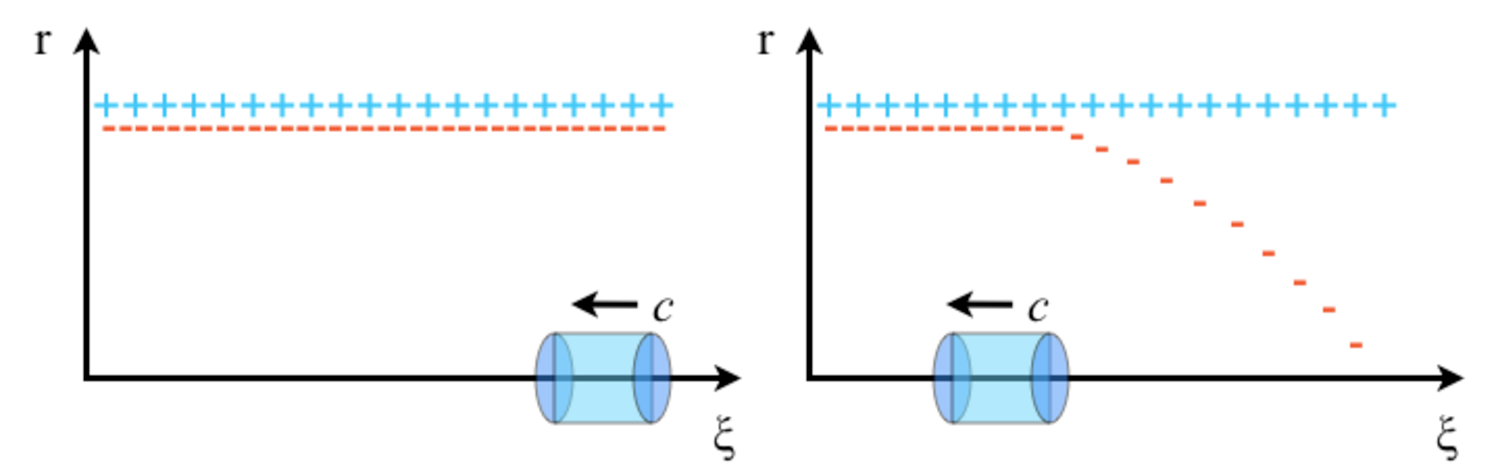
\includegraphics[width=150mm]{./figures/thin_cyl.pdf}
      \caption{A thin cylinder plasma with a flat top drive beam.}
\end{figure}

The plasma profile is $\rho_p = \lambda \delta(r - a)$ and the beam has a width $\sigma_r \ll a$, length $L \ll \lambda_p$, energy $\gamma$, and charge density $n_b$. The beam field at the plasma radius is $E_b = 2\pi \gamma n_b \sigma_r^2/a$. The plasma feels a kick per unit length from the beam given by $\Delta p = c E_b \lambda/L$ and this kick causes the plasma electrons to drift inward from the plasma ions. We now seek an equation of motion for the position of the plasma electron sheath $r_s$. We assume the ions are stationary.

First, we solve for the potential $\phi$ and we take $\phi(\infty) = 0$. Outside the cylinder, there is zero net charge (after the drive beam has passed), so Gauss's law gives $E(r > a) = 0$ and therefore $\phi(r > a) = const = 0$. Inside the electron sheath there is no charge either, so $E(r < r_s) = 0$ and $\phi(r < r_s) = \phi_0$. Between the electron sheath and the ion layer there is a net charge and Gauss's law gives $E(r) = 2\lambda/r$ for $r_s < r < a$. We can now find the potential by integrating the electric field:

\begin{equation}\label{eq:thin_phi}
\phi(r) = -\int_0^r E(r') dr' = \phi_0 - \int_{r_s}^r \frac{2\lambda}{r'}dr' = \phi_0 + 2\lambda \log\left(\frac{r_s}{r}\right)
\end{equation}

Using the boundary condition $\phi(a) = 0$ we find that $\phi_0 = 2\lambda \log\left(\frac{a}{r_s}\right)$ so:

\begin{equation}\label{eq:phi_everywhere}
\phi(r) = \left\{ \begin{array}{lr}
2\lambda \log\left(\frac{a}{r_s}\right) & 0<r<r_s \\
2\lambda \log\left(\frac{a}{r_s}\right) + 2\lambda \log\left(\frac{r_s}{r}\right) & r_s<r<a \\
0 & a<r
\end{array} \right.
\end{equation}

\begin{figure}[ht]\label{fig:fields}
  \centering
    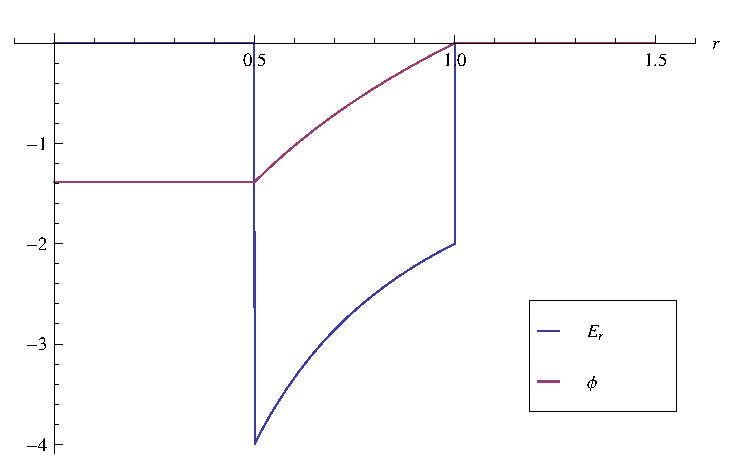
\includegraphics[width=100mm]{./figures/fields.pdf}
      \caption{$E_r$ and $\phi$ for the thin cylinder model. $\lambda = -1$ and distances are normalized to $a=1$.}
\end{figure}

Next, we find $\mathbf{A}_{\perp}$ using equation~\ref{eq:gauge_qs} and assuming that the motion of the plasma electrons is purely radial so $A_z = 0$ and $\psi = \phi$. Then

\begin{equation}\label{eq:a_perp}
\nabla_\perp \cdot \mathbf{A}_\perp = -\frac{\partial \phi}{\partial \xi} = - \frac{\partial \phi}{\partial r_s}\frac{\partial r_s}{\partial \xi} = \frac{2\lambda}{r_s}r_s'
\end{equation}

In cylindrical coordinates, the divergence is

\begin{equation}\label{eq:a_perp_cyl}
\nabla_\perp \cdot \mathbf{A}_\perp = \frac{1}{r}\frac{\partial}{\partial r} (r A_r) + \frac{1}{r}\frac{\partial A_{\theta}}{\partial \theta}
\end{equation}

but we drop the $\theta$ term due to the cylindrical symmetry. We note that $r$ and $r_s$ are independent variables in this equation so we can easily integrate the equation in $r$ to find $A_r$

\begin{equation}\label{eq:a_r}
\frac{1}{r}\frac{\partial}{\partial r} (r A_r) = \frac{2\lambda}{r_s}r_s' \rightarrow A_r = \frac{\lambda r r_s'}{r_s}
\end{equation}

At this point, we'd like to start determining some physical quantities of interest, like $E_z$

\begin{equation}\label{eq:E_z}
E_z = \frac{\partial \psi}{\partial \xi} = -\frac{2\lambda}{r_s}r_s'
\end{equation}

so we need an equation of motion for $r_s$. We can get the EOM by finding the force on the plasma electrons in the sheath:

\begin{equation}\label{eq:force}
F =-(E_r -V_z B_{\theta}) = -E_r
\end{equation}

because we have assumed that $V_z = 0$. The radial field is

\begin{equation}\label{eq:force}
E_r =-\nabla_{\perp} \phi - \frac{\partial A_r}{\partial \xi} = -\frac{\lambda r}{r_s^2}[r_s r_s'' - r_s'^2]
\end{equation}

with $\nabla_{\perp} \phi = 0$ for the sheath electrons because there is zero charge within the sheath layer. The EOM $\partial_{\xi} P_{\perp} = -E_r$ can be rewritten using the integral of motion $\gamma - P_z = 1 + \psi$:

\begin{equation}\label{eq:EOM}
\frac{\partial P_{\perp}}{\partial \xi} = \frac{\partial}{\partial \xi}[(1+\psi)r_s'] = \frac{\lambda r}{r_s^2}[r_s r_s'' - r_s'^2] 
\end{equation}

Plugging in $\psi = \phi$ we have:

\begin{equation}\label{eq:rs}
\left(1+2\lambda\log\left(\frac{a}{r_s}\right) - \lambda\right)r_s'' -\lambda\frac{r_s'^2}{r_s} = 0
\end{equation}

In order to study this equation, let's set $a=1$ and $\lambda = -1$. Then

\begin{equation}\label{eq:rs_simp}
(2+2\log(r_s)) r_s r_s'' + r_s'^2 = 0
\end{equation}

Immediately we see that we might run into trouble when $r_s = 0$ due to the divergence in the log term (although $x\log x = 0$ as $x\rightarrow0$).

\begin{figure}[ht]\label{fig:sheath}
  \centering
    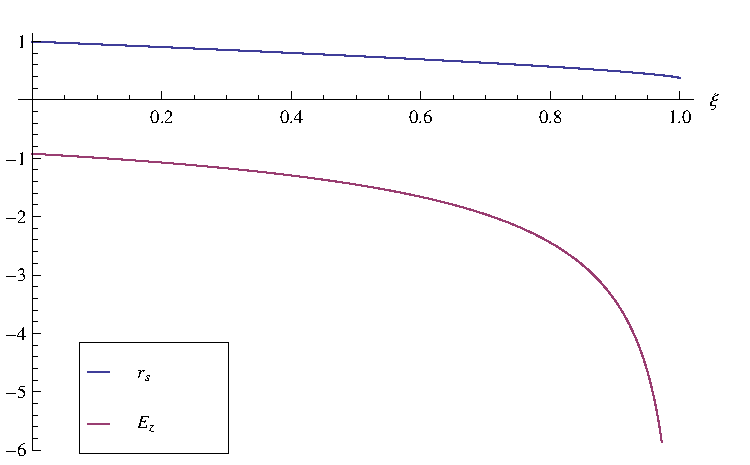
\includegraphics[width=100mm]{./figures/sheath.pdf}
      \caption{$r_s$ and $E_z$ for the thin cylinder model. $\lambda = -1$ and distances are normalized to $a=1$. The initial kick $r_s'(0) = -0.46$. This is the largest kick that Mathematica can use to solve the equation for the given plot range.}
\end{figure}

\subsection{Adding in longitudinal plasma motion}


\end{document}